\documentclass{article}
\usepackage[utf8]{inputenc}
\usepackage{graphicx}
\bibliographystyle{plain}

\title{libbdsg and libhandlegraph: High-performance sequence graph implementations for graphical pangenomics}
\author{Jordan M. Eizenga \and Adam M. Novak \and Emily Kobayashi \and Cecilia Cisar \and Benedict Paten \and Erik Garrison}

\newcommand{\vocab}{\textbf}

\begin{document}

\maketitle

\begin{abstract}

Pangenomics is a growing field within computational genomics \cite{computational2016computational}. Many pangenomic analyses use bidirected sequence graphs as their core data model. However, implementing and correctly using this data model can be difficult, and the scale of pangenomic data sets can be challenging to work with. Here we present two C++ libraries with Python bindings, \texttt{libbdsg} and \texttt{libhandlegraph}. They provide a suite of high-performance sequence graph implementations, ready for use in user applications. Additionally, they share a simple, field-proven interface designed to prevent common graph manipulation mistakes.

\end{abstract}

\section{Introduction}

With falling sequencing costs, the genomics community has sequenced increasingly many individuals within certain species. For example, hundreds of thousands of deeply sequenced human genomes are now available. The novel challenges of analyzing data sets of this scale have led to the development of \vocab{computational pangenomics}: the analysis of populations of genomes rather than individuals.

Much of the research in computational pangenomics has coalesced around graph-based approaches for representing populations of genomes. Unlike conventional string-based representations, graph data structures provide a modeling language to represent different types of genomic variation like substitutions, insertions, deletions, and more complex genomic events. 

Graph-based data structures also present new computational challenges. In addition to sequence, graphs must represent topology. Given the size of many genomes of interest, this can be quite demanding on computer memory. Further, there is significant impetus to make the graph data structures computationally efficient, since they are frequently the core data structure in pangenomics applications.

We have developed a stack of C++ libraries providing high-performance sequence graphs for graphical pangenomics applications. We also provide Python bindings so the components are accessible to Python developers as well. This resource will reduce the need for individual research groups to continually reimplement these core data structures. The C++ stack consists of two components. First, we have developed an abstract interface for sequence graphs, based on our experience in the VG project. Second, we have developed three concrete implementations of the sequence graph interface, which make different trade-offs between speed, memory, and complexity, and which attempt to provide good coverage of the design space. 

\section{Implementation}

\subsection{Data model}

Our libraries adopt node-labeled bidirected graphs as a formalism for sequence graphs. In a bidirected graph, nodes are considered to have left and right ``sides'', and edges connect two sides rather than two nodes. In bidirected sequence graphs, a node's sides correspond to the 5' and 3' ends of its DNA sequence. 

Paths through a bidirected graph must leave a node out of the opposite side that they enter it. We interpret paths that traverse a node from the 3' side to the 5' as using the node's reverse complement strand, which provides a natural means to encode DNA strandedness. Specific paths correspond to sequences of interest, such as reference genomes. Because paths like these are so frequently important in practice, our formalism also includes paths as a first class object, embedded in the graph.

\subsection{The handle graph interface}

The \texttt{libhandlegraph} library describes a generic interface that exposes basic operations on our sequence graph data model. The interface uses ``handles'', modeled after the concept of the file handle, in order to remain agnostic about the backing implementation of the graph. That is, the interface requires sequence graph implementations to be able to provide handles to important graph features such as oriented nodes, paths, and steps in paths. The handles are then passed back to the graph to refer to these entities when performing operations and making queries. The actual contents of a handle are unspecified, which gives significant flexibility to the implementation.

One benefit of this design is that any algorithm designed for one handle graph implementation can be applied to all other implementations. Another is that, since the user works only through handles, their ability to make mistakes can be restricted. For example, the interface can enforce the constraints on paths through bidirected graphs during edge traversal. This prevents common mistakes that the developers identified in their work on the VG project. Taken together, these benefits enable code that focuses on the algorithms rather than on boilerplate bookkeeping.

\subsection{Graph implementations}

The \texttt{libbdsg} library consists of four concrete implementations of the handle graph interface. Each implementation represents a different tradeoff in terms of speed, memory use, and capabilities. All of the implementations except XG are dynamic.

\subsubsection{HashGraph}

This implementation has speed as its primary goal. The core adjacency list is implemented using a high performance hash table. Most of the smaller component data structures are uncompressed STL objects, so they can easily be computed on in the native in-memory format. Embedded paths are implemented as doubly-linked lists. This implementation is most appropriate for small graphs (from small genomes or small regions of larger genomes) or for high-memory compute environments.

\subsubsection{PackedGraph}

This implementation focuses on having a low memory footprint. Most of its component data structures are---conceptually speaking---linked lists. However, they are implemented using vectors of bit-compressed integers, where pointers are produced by treating some of the integer entries as indexes into the vector that contains them. The bit-width can be chosen dynamically without affecting the amortized asymptotic run time of graph operations in the typical case that the $i$-th entry in the vector is $O(i)$. The vector uses a windowed bit compression scheme in which only one value within a window is maintained at its full bit-width. The remaining entries are represented as differences from this value. In the typical case where adjacent entries in the vector are highly correlated, this helps keep the bit-width low and thereby the compression high. 

\subsubsection{ODGI}

TODO: brief description of implementation

\subsubsection{XG}

Unlike the others, this implementation is static. This permits a more powerful set of efficient queries from the graph, especially from paths. The encoding is designed to balance speed and low-memory usage. The topology of the graph is encoded in a single vector of bit-compressed integers, which promotes cache-efficiency. Rank and select operations on compressed bit-vectors are used to provide random access over the variable-width records. Embedded paths are encoded in variable-length integer vectors with Elias gamma encoding. Rank and select operations from bit vectors also provide queries by base-pair position along paths.

\section{Evaluation}

We measured the performance during core operations of the four graph implementations and the graph class from the popular VG software. In particular, we measured 1) memory usage while constructing a graph, 2) time to construct a graph, 3) memory usage when loading an already-constructed graph, and 4) time to access nodes, edges, and steps of a path. The presented results are from a graph constructed from the structural variants of the HGSVC. The comparison generally follows our expectations based on the design principles behind each implementation (Figure \ref{fig:hgsvc}).

\begin{figure}
	\begin{center}
		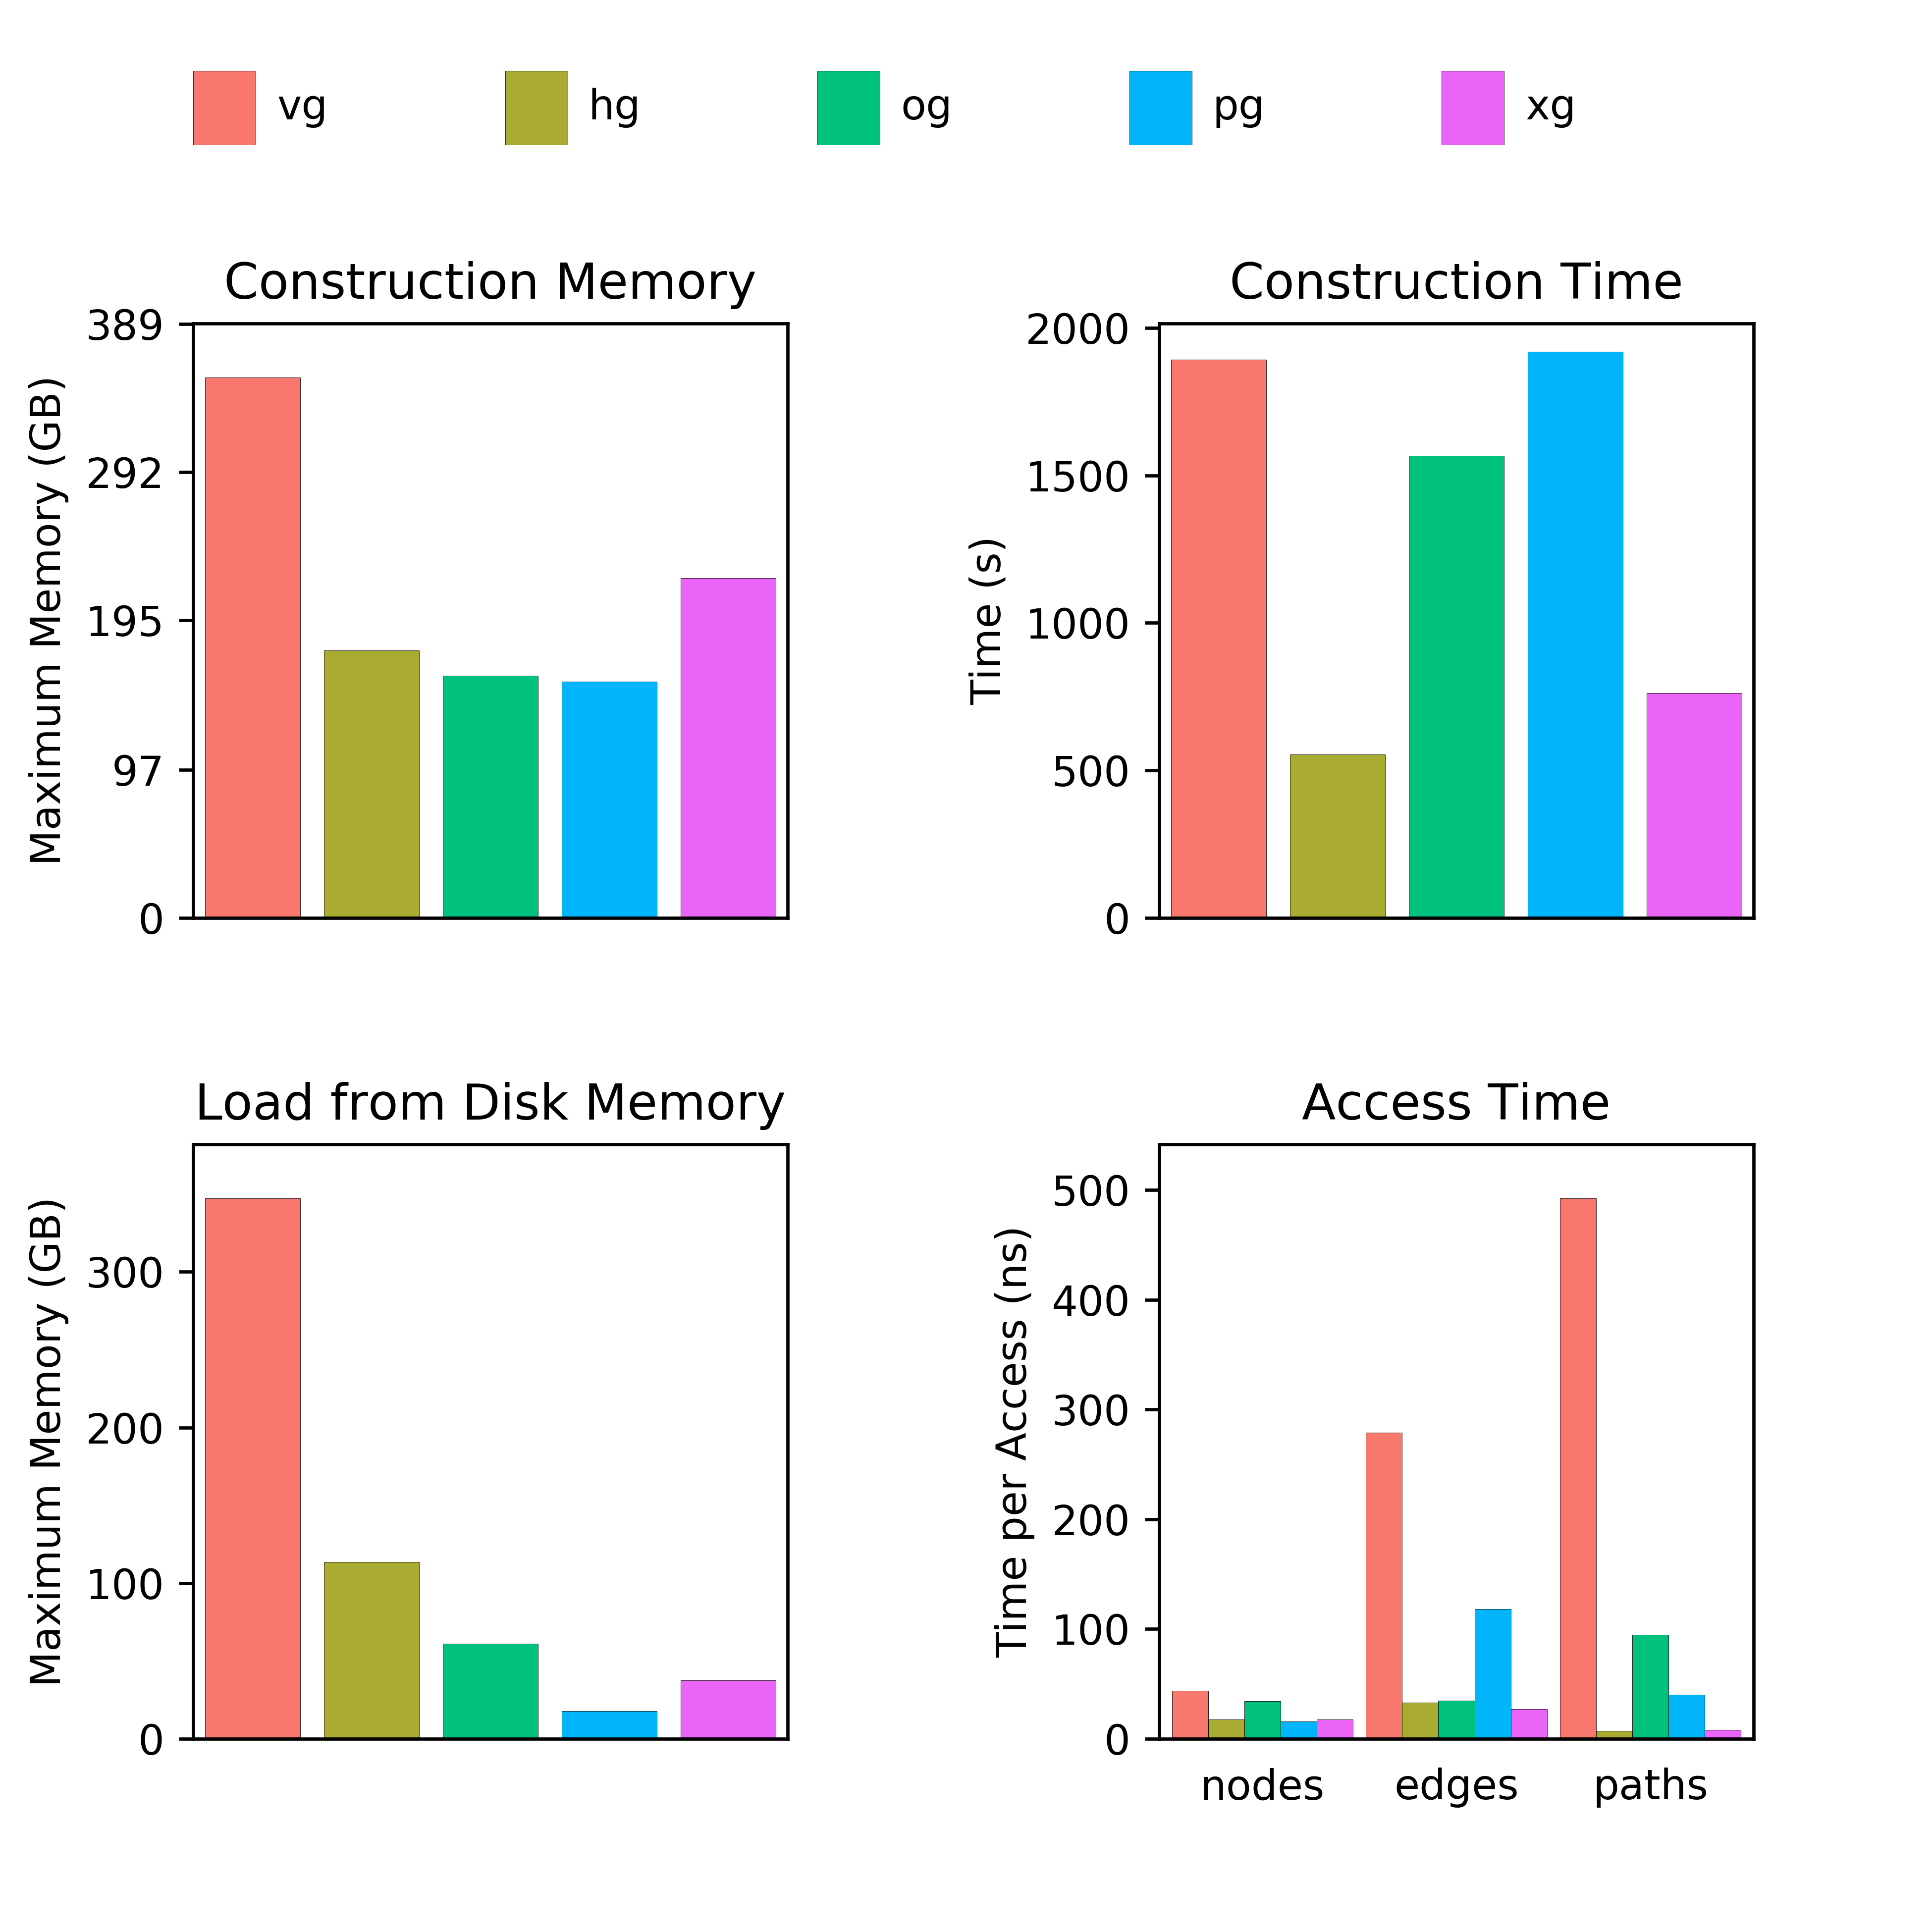
\includegraphics[width=.75\textwidth]{figures/HGSVC_sorted_gfa.png}
	\end{center}
	\caption{{\label{fig:hgsvc} \textbf{Performance on a graph of structural variants from the HGSVC.} All four new graph implementations compare favorably to VG. PackedGraph tends to be the most memory efficient, HashGraph tends to be the fastest, and ODGI is balanced in between. XG provides good performance on both memory usage and speed, but it is static.}}
\end{figure}

% \section{Discussion}

% The \texttt{libhandlegraph} and \texttt{libbdsg} C++ libraries provide high-performance sequence graph implementations that encourage quality coding. Python bindings are also available. This software can help developers write future pangenomics applications. 

% TODO: we should write a guide on GitHub for how to use

\bibliography{references.bib}

\end{document}
